\thispagestyle{diendandayvahoctoannone}
\pagestyle{diendandayvahoctoan}
\everymath{\color{diendantoanhoc}}
\graphicspath{{../diendantoanhoc/pic/}}
%\blfootnote{$^{1}$\color[named]{diendantoanhoc}Hà Nội.}
\begingroup
\AddToShipoutPicture*{\put(0,616){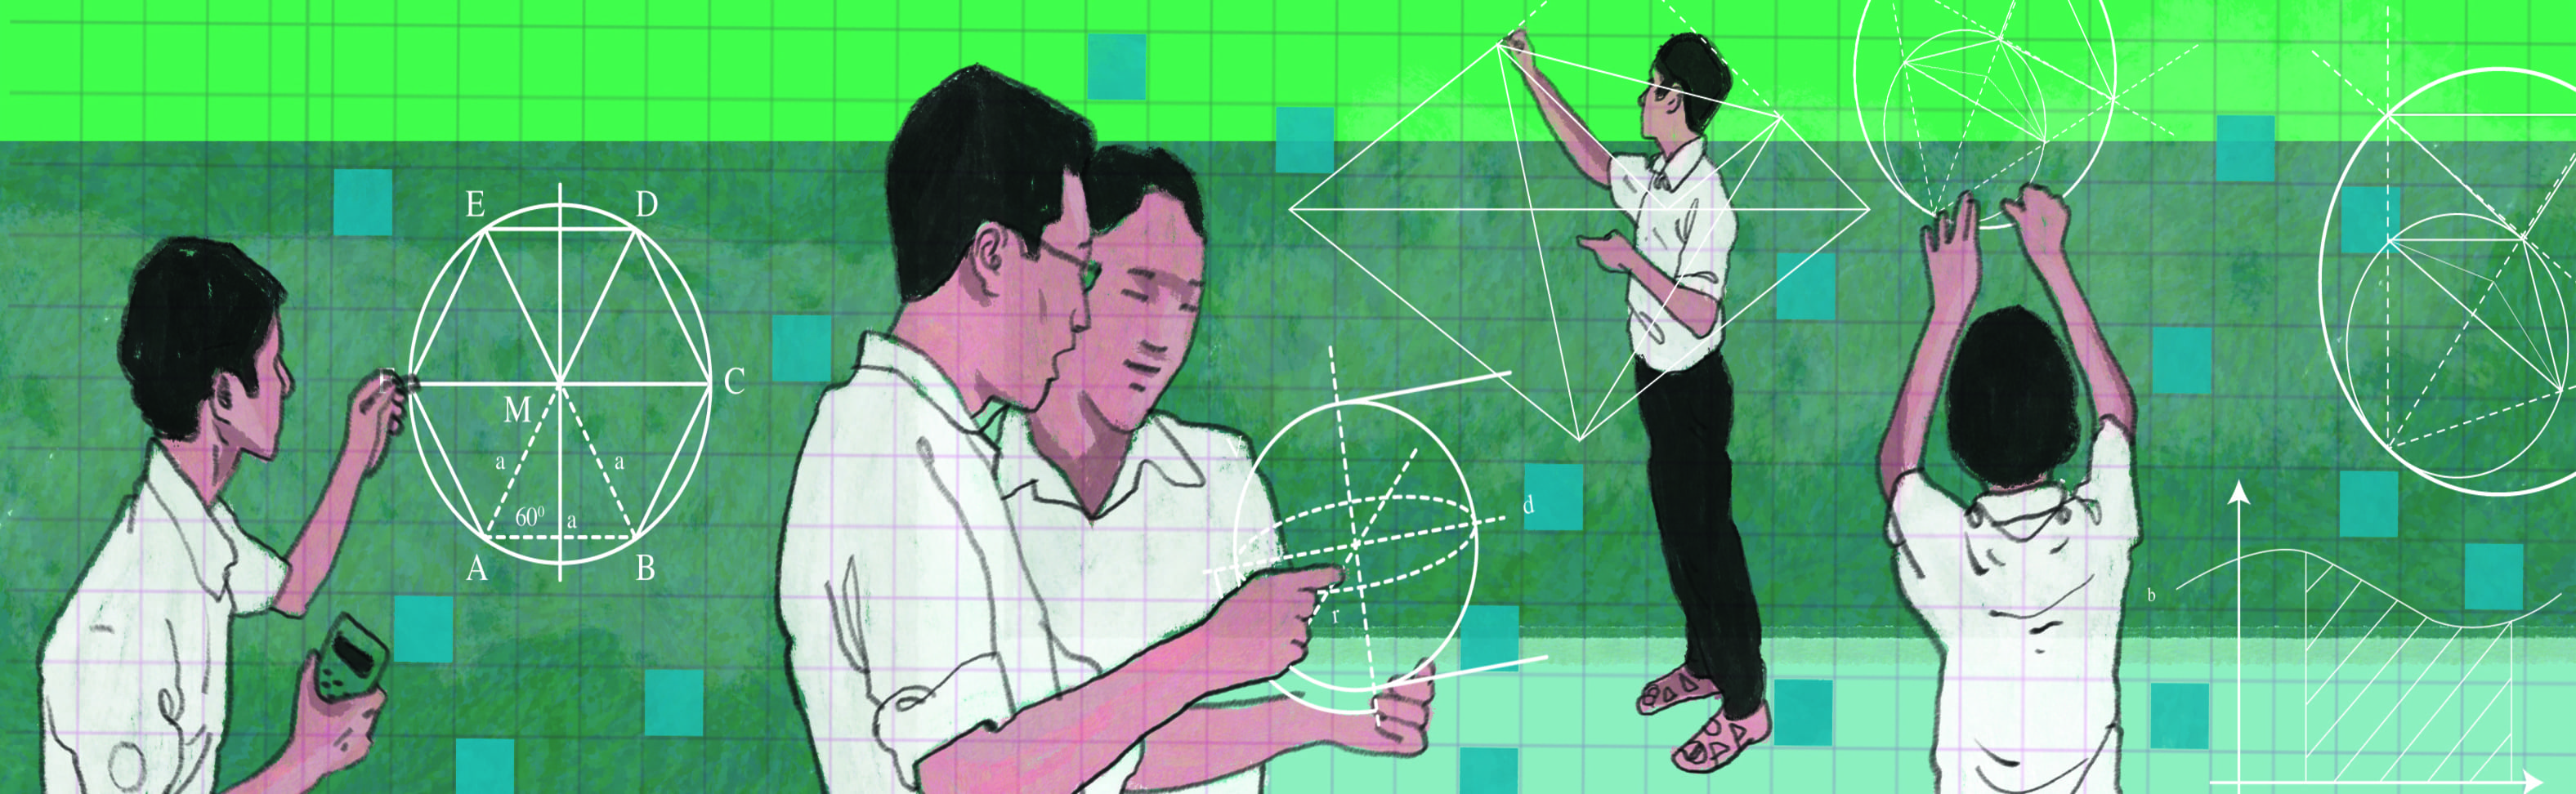
\includegraphics[width=19.3cm]{../bannerdiendan}}}
\AddToShipoutPicture*{\put(78,553){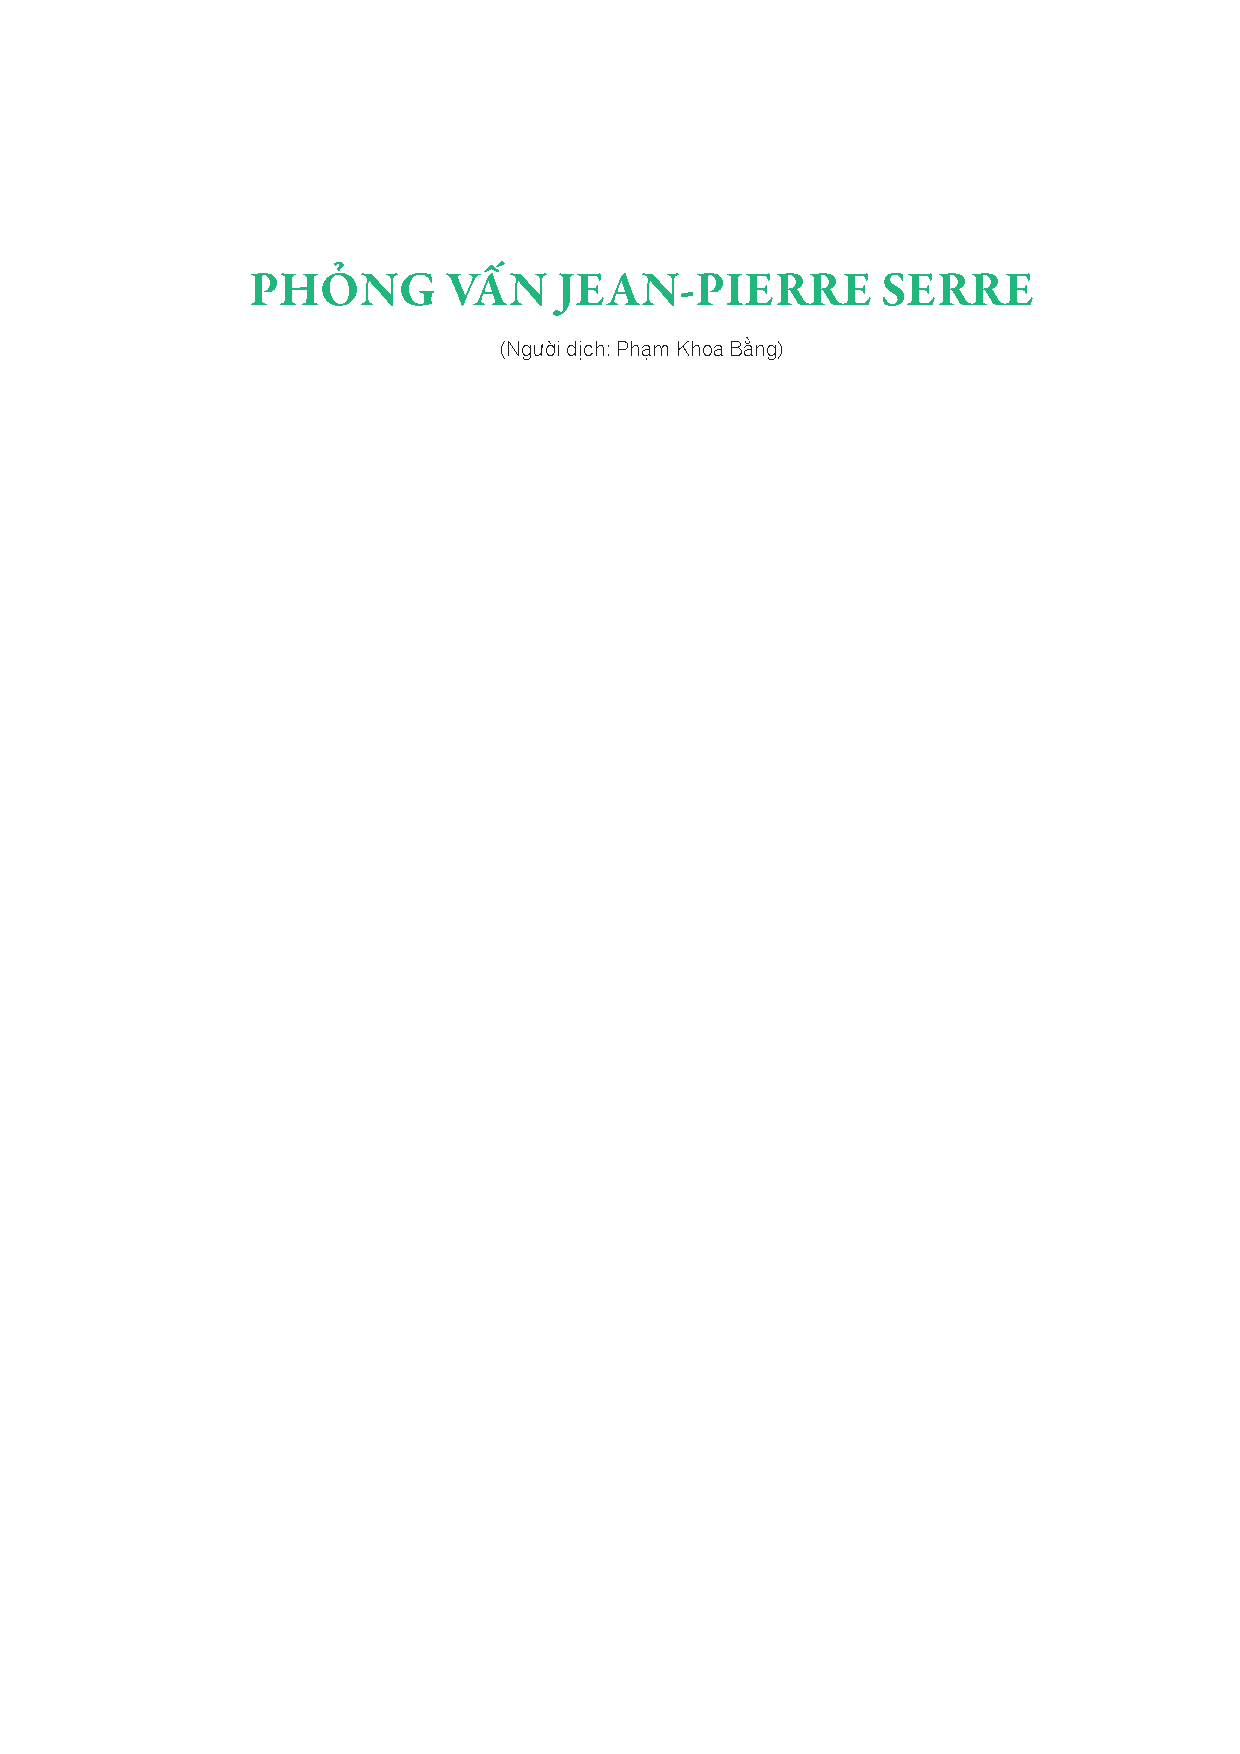
\includegraphics[scale=1]{../tieude2.pdf}}}
\centering
\endgroup
\vspace*{155pt}

\begin{multicols}{2}
	Jean--Pierre Serre sinh năm $1926$ tại Pháp. Ông từng theo học toán tại đại học sư phạm Paris. Vào năm $1954$, ở tuổi $28$, ông đã được giải Fields bởi Hiệp hội Toán học Quốc tế, chứng nhận cao nhất cho một thành tựu trong toán học. Hai năm sau ông được bổ nhiệm chức Giáo sư về Đại số và Hình học tại College de France, nơi mà ông là giáo sư trẻ nhất trong khoảng $15$ năm. Ông thăm khoa toán Đại học Quốc Gia Singapore từ ngày $2$ tới $15$ tháng Hai năm $1985$. Chuyến thăm của ông được tài trợ chương trình trao đổi học thuật Pháp--Sing. Khi ở Singapore, giáo sư Serre đã trình bày hai bài giảng về đường cong đại số trên trường hữu hạn và một bài giảng về hàm Ramanujan. Ông cũng góp một bài nói seminar hai tiếng về chứng minh của Faltings cho giả thuyết Mordell, và một bài giảng hội đàm với tiêu đề ``Biệt thức = $b^2-4ac$" về ``class numbers" của các trường toàn phương ảo. Vào ngày $14$ tháng Hai năm $1985$, ông có một cuộc phỏng vấn trong đó ông thảo luận nhiều khía cạnh trong sự nghiệp toán học của mình và cách nhìn của ông về toán học. Những gì sau đây là ghi chép từ cuộc phỏng vấn đó, chỉnh sửa bởi C. T. Chong và Y. K. Leong, và đã được kiểm tra lại bởi J. P. Serre.
	Q: Điều gì khiến ông chọn toán học làm sự nghiệp của mình?
	\vskip 0.1cm
	A: Tôi nhớ rằng tôi bắt đầu thích toán vào khoảng năm $7$ hoặc $8$ tuổi. Hồi còn trung học tôi thường giải các bài toán của các lớp lớn hơn. Hồi ấy tôi ở một khu nhà trọ ở Nimes cùng với lũ trẻ lớn hơn và chúng thường bắt nạt tôi. Để làm hoà với chúng, tôi thường làm hộ bài tập về nhà môn toán cho chúng. Dù sao đó cũng là một bài luyện tập tốt.
	\vskip 0.1cm
	Mẹ tôi là một dược sĩ (cũng như bố tôi), và bà yêu toán học. Khi bà ấy vẫn còn là một sinh viên dược tại đại học Montpellier, bà ấy đã đăng ký học một khoá học năm đầu tiên môn giải tích, chỉ để cho vui, và bà đã vượt qua bài kiểm tra. Và bà ấy đã giữ cẩn thận những quyển sách giải tích của mình (viết bởi Fabry và Vogt, nếu tôi nhớ không nhầm). Khi tôi $14$ hoặc $15$, tôi thường xem những quyển sách này và nghiên cứu chúng. Đó là cách tôi học về đạo hàm, tích phân, chuỗi và các thứ kiểu thế (tôi học theo một cung cách hình thức thuần tuý -- phong cách của Euler với tôi mà nói thì tôi không thích, và không hiểu ngôn ngữ epsilon delta.) Vào thời điểm đó, tôi không biết rằng người ta có thể kiếm sống bằng cách trở thành một nhà toán học. Chỉ sau này tôi mới khám phá ra rằng người ta được trả tiền để làm toán! Đầu tiên tôi nghĩ tôi sẽ trở thành một giáo viên trung học, điều đó dường như là tự nhiên với tôi. Nhưng khi tôi $19$, tôi đã đăng ký kì thi vào trường Đại học Sư phạm Paris và tôi thành công. Khi tôi đã ở trong ``Trường", tôi thấy rõ rằng không phải giáo viên trung học là cái tôi muốn trở thành, mà tôi muốn trở thành một nhà toán học.
	\vskip 0.1cm
	Q: Những lĩnh vực khác có từng thu hút ông không, như vật lý hoặc hoá học?
	\vskip 0.1cm
	A: Vật lý thì không nhiều lắm, nhưng hoá học thì có đấy. Như tôi đã nói, bố mẹ tôi đều là dược sĩ, nên họ có cả đống hoá chất và ống nghiệm. Tôi nghịch chúng rất nhiều khi tôi mới $15$ $16$ ngoài việc làm toán. Và tôi đọc những quyển sách hoá học của bố tôi (tôi vẫn giữ một trong số chúng, một quyển sách lôi cuốn, ``Les Colloides" của Jacques Duclaux). Tuy nhiên, khi học thêm hoá, tôi thất vọng vì cái khía cạnh gần như toán học của nó: có một chuỗi các hợp chất hữu cơ như $CH_4,C_2H_6,...$, tất cả đều ít nhiều giống nhau. Tôi nghĩ, nếu mà phải có chuỗi thì thà tôi đi làm toán! Do đó tôi từ bỏ hoá học -- nhưng không hoàn toàn: cuối cùng tôi cưới một nhà hoá học.
	\vskip 0.1cm
	Q: Ông có từng bị ảnh hưởng bởi giáo viên học đường nào trong việc làm toán không?
	\vskip 0.1cm
	A: Tôi chỉ từng có đúng một giáo viên rất tốt. Đó là năm cuối của tôi ở trường trung học ($1943-1944$), ở Nimes. Ông ấy có biệt danh ``Le Barbu": để râu rất hiếm vào thời đó. Ông ấy luôn rất rõ ràng, và chặt chẽ; ông ấy yêu cầu mọi công thức và chứng minh phải được trình bày gọn gàng. Và ông ấy đã dành cho tôi một bài luyện tập tận tâm cho kỳ thi toán học quốc gia có tên ``Concours General", nơi mà cuối cùng tôi dành giải nhất.
	\vskip 0.1cm
	Nói về Concours General, tôi cũng thử với tay mình sang kỳ thi đó bên vật lý, vào cùng năm ($1944$). Vấn đề chúng tôi được hỏi hoàn toàn dựa vào một định luật vật lý mà tôi nên biết, nhưng tôi lại không biết nó. May mắn thay, chỉ có một công thức dường như có thể áp dụng cho định luật đó. Tôi đã giả sử nó đúng, và triển khai làm việc với một vấn đề $6$--tiếng dựa trên giả sử đó. Tôi thậm chí còn nghĩ mình sẽ đạt giải. Không may mắn lắm, công thức của tôi sai, và tôi không đạt được gì -- điều mà tôi xứng đáng!
	\vskip 0.1cm
	Q: Cảm hứng có vai trò quan trọng như thế nào trong việc tìm ra các định lý?
	\vskip 0.1cm
	A: Tôi không biết ``cảm hứng" thực sự có nghĩa gì. Các định lý và các lý thuyết đến theo những cách buồn cười. Thỉnh thoảng, anh chỉ không hài lòng với các chứng minh đã có, và anh tìm những chứng minh tốt hơn để có thể áp dụng cho các tình huống khác. Một ví dụ điển hình với tôi là khi tôi làm việc với định lý Riemann--Roch (khoảng năm $1953$), mà tôi xem nó như một công thức ``Euler--Poincaré" (tôi đã không biết rằng Kodaira--Spencer đã có cùng ý tưởng.) Mục tiêu đầu tiên của tôi là chứng minh nó cho các đường cong đại số -- một trường hợp đã biết từ cả thế kỷ trước! Nhưng tôi muốn một chứng minh theo một phong cách đặc biệt, và khi tôi thành công trong việc tìm ra nó, tôi nhớ rằng tôi mất không quá một hoặc hai phút để đi từ đó lên trường hợp $2$ chiều (điều chỉ vừa được chứng minh bởi Kodaira). Sáu tháng sau, kết quả hoàn chỉnh được đưa ra bởi Hirzebruch, và công bố trong bài Habilitationsschrift nổi tiếng của ông ấy.
	\vskip 0.1cm
	Thông thường, anh không giải quyết một vấn đề bằng cách tấn công trực diện nó. Thay vào đó anh có vài ý tưởng trong đầu mà anh cảm giác sẽ có ích, nhưng anh không thật sự biết chính xác rằng chúng có ích cho điều gì. Do đó, anh tìm kiếm xung quanh, và cố gắng áp dụng chúng. Giống như việc có cả chùm chìa khoá, và cố gắng thử chúng vào những cái cửa.
	\vskip 0.1cm
	Q: Ông có từng có trải nghiệm nào mà ông thấy một vấn đề là không thể giải quyết, nhưng sau khi bỏ nó sang một bên một thời gian thì một ý tưởng đột nhiên xuất hiện dẫn tới lời giải không?
	\vskip 0.1cm
	A: Có, chắc chắn điều này vẫn thường diễn ra. Ví dụ, khi tôi làm việc với các nhóm đồng luân (khoảng năm $1950$), tôi tự thuyết phục mình rằng, với một không gian $X$, nên tồn tại một không gian phân thớ $E$, với nền $X$, mà có thể co rút về một điểm; một không gian như thế có thể cho phép tôi (sử dụng các phương pháp của Leray) làm rất nhiều các tính toán về nhóm đồng luân và đối đồng điều của không gian Eilenberg--MacLane. Nhưng làm thế nào để tìm ra nó? Tốn vài tuần (một thời gian rất dài, vào cái tuổi tôi lúc đó...) để tôi nhận ra không gian các ``đường" trên $X$ có đủ các tính chất cần thiết -- chỉ khi tôi dám gọi nó là ``không gian phân thớ", và tôi đã làm vậy. Đây là điểm bắt đầu của phương pháp không gian cung trong tôpô đại số, rất nhiều kết quả sau đó nhanh chóng được chứng minh.
	\vskip 0.1cm
	Q: Ông thường làm việc với chỉ một vấn đề hay nhiều vấn đề cùng lúc?
	\vskip 0.1cm
	A: Hầu như chỉ một vấn đề từng thời điểm, nhưng không phải luôn luôn. Và tôi thường làm việc buổi đêm (giấc ngủ chập chờn), khi mà anh không phải viết thứ gì ra sẽ làm cho đầu óc có độ tập trung cao hơn, và thay đổi các chủ đề dễ dàng hơn.
	\vskip 0.1cm
	Q: Trong vật lý, có rất nhiều khám phá là do tình cờ, ví dụ như tia X, bức xạ nền vũ trụ, vân vân. Điều đó có xảy ra với ông trong toán học?
	\vskip 0.1cm
	A: Một sự tình cờ thật sự là rất hiếm. Nhưng thi thoảng anh vẫn ngạc nhiên vì một lập luận của anh cho một mục đích lại có thể giải quyết một câu hỏi trong một hướng nghiên cứu khác; tuy nhiên, người ta khó có thể gọi nó là "tình cờ".
	\vskip 0.1cm
	Q: Đâu là những vấn đề cốt lõi trong hình học đại số và lý thuyết số?
	\vskip 0.1cm
	A: Tôi không thể trả lời chính xác. Anh thấy đấy, vài nhà toán học có những ``chương trình" rõ ràng và dài hơi. Ví dụ, Grothendieck có một chương trình như thế cho hình học đại số; bây giờ Langlands có một cái như vậy cho lý thuyết biểu diễn, trong mối quan hệ với dạng modular và số học. Tôi chưa từng có một chương trình như vậy, kể cả một cái cỡ nhỏ. Tôi chỉ làm việc với những thứ hấp dẫn tôi tại một thời điểm. (hiện tại, vấn đề hấp dẫn tôi nhất là đếm số điểm trên các đường cong đại số trên những trường hữu hạn. Nó là một kiểu toán ứng dụng: anh cố sử dụng bất kỳ công cụ nào trong hình học đại số và lý thuyết số mà anh biết... và anh không thành công lắm!)
	\vskip 0.1cm
	Q: Ông cho rằng đâu là những tiến bộ vượt bậc nhất trong hình học đại số và lý thuyết số trong vòng năm năm trở lại đây?
	\vskip 0.1cm
	A: Câu này dễ trả lời hơn. Chứng minh của Falting cho giả thuyết Mordell và giả thuyết Tate là điều đầu tiên tôi nghĩ đến. Tôi cũng xin nhắc đến công trình của Gross--Zagier về vấn đề số lớp (class number problem) cho các trường toàn phương (dựa trên một định lý trước đó của Goldfeld), và định lý Mazur--Wiles về lý thuyết Iwasawa, sử dụng đường cong modular. (Những ứng dụng của các đường cong modular và các hàm modular vào lý thuyết số là cực kỳ thú vị: anh sử dụng $GL_2$ để nghiên cứu $GL_1$, có thể nói như vậy! Rõ ràng là còn rất nhiều thứ sẽ tới theo hướng đó... thậm chí có thể là chứng minh giả thuyết Riemann vào một ngày nào đó!) 
	\vskip 0.1cm
	Q: Vài nhà khoa học đã làm được một số công trình nền tảng trong một lĩnh vực và sau đó nhanh chóng chuyển sang lĩnh vực khác. Ông đã làm việc ba năm với tôpô, và sau đó làm thứ khác. Điều đó đã xảy ra như thế nào?
	\vskip 0.1cm
	A: Nó là một con đường liền mạch, không phải một thay đổi rời rạc. Năm $1952$, sau luận án của tôi về các nhóm đồng luân, tôi đến Princeton nơi mà tôi có bài giảng về luận án của mình (và phần tiếp theo của nó: ``lý thuyết C"), và tham dự seminar nổi tiếng Artin--Tate về lý thuyết trường các lớp. 
	\vskip 0.1cm
	Sau đó tôi trở về Paris, nơi mà seminar Cartan đang thảo luận về các hàm phức nhiều biến, và các đa tạp Stein. Hoá ra các kết quả gần đây của Cartan--Oka có thể được biểu diễn hiệu quả hơn (và được chứng minh theo cách đơn giản hơn) nhờ sử dụng đối đồng điều và bó. Điều đó khá phấn khích, và tôi đã làm việc một thời gian ngắn về chủ đề này, áp dụng lý thuyết Cartan vào các đa tạp Stein. Tuy nhiên, một mảng thú vị của lý thuyết hàm phức nhiều biến là nghiên cứu các đa tạp xạ ảnh (đối lập với các đa tạp affine -- được xem là khá bệnh hoạn với một nhà hình học); bởi vậy tôi bắt đầu làm việc với các đa tạp xạ ảnh phức, sử dụng bó: đó là cách tôi đến với cái vòng các ý tưởng xung quanh Riemann--Roch vào năm $1953$. Nhưng các đa tạp xạ ảnh thì đại số (định lý Chow), và nó hơi thiếu tự nhiên nếu muốn nghiên cứu những đối tượng đại số này bằng các hàm giải tích, vốn có thể có rất nhiều kỳ dị không bỏ được. Rõ ràng, chỉ nên làm với các hàm hữu tỷ là đủ -- và đúng là như vậy. Điều đó đưa tôi (vào khoảng năm $1954$) đến với hình học đại số ``trừu tượng", trên bất kỳ trường đóng đại số nào. Nhưng tại sao phải giả sử trường là đóng đại số? Các trường hữu hạn thú vị hơn, với giả thuyết Weil và những thứ tương tự. Và từ đó đến với những trường số, đó là một bước chuyển tiếp tự nhiên... Đây ít nhiều là con đường tôi đã theo đuổi. 
	\vskip 0.1cm
	Một hướng nghiên cứu khác đến tự sự hợp tác (và tình bạn) của tôi với Armand Borel. Ông ấy nói về tôi về nhóm Lie, thứ mà ông ấy biết như rõ hơn bất kỳ ai. Mối liên hệ giữa những nhóm này với tôpô, hình học đại số, lý thuyết số,... là rất lôi cuốn. Để tôi cho anh một ví dụ (mà tôi để ý vào khoảng năm $1968$):
	\vskip 0.1cm 
	Hãy xem xét nhóm con rời rạc hiển nhiên nhất của $\mathrm{SL}_2(\mathbf{R})$, tức là $\Gamma = \mathrm{SL}_2(\mathbf{Z})$. Anh có thể tính ``đặc trưng Euler--Poincare" $\chi(\Gamma)$ của nó và nó bằng $-1/12$ (nó không phải là số nguyên, bởi vì $\Gamma$ có xoắn). Giờ anh thấy $-1/12$ là giá trị $\zeta(-1)$ của hàm Riemann--zeta tại $s=-1$ (một kết quả biết từ thời Euler). Và đây không phải là sự trùng hợp! Nó mở rộng lên bất kỳ trường số thực hoàn toàn $K$ nào (totally real number field), và có thể sử dụng để nghiên cứu mẫu số của $\zeta_k(-1)$. (Các kết quả tốt hơn thu được bằng cách sử dụng dạng modular, như sau này được tìm ra.) Những câu hỏi như thế không phải lý thuyết nhóm, không phải tôpô, cũng chẳng phải lý thuyết số: chúng chỉ là toán học.
	\vskip 0.1cm
	Q: Đâu là những triển vọng trong việc đạt được vài sự thống nhất các lĩnh vực toán học đa dạng?
	\vskip 0.1cm
	A: Tôi có thể nói điều này đã đạt được rồi. Tôi đã đưa ra bên trên một ví dụ điển hình về nhóm Lie, lý thuyết số, vân vân, đến cùng nhau và không thể bị tách rời. Để tôi cho anh một ví dụ khác (và không khó để đưa ra thêm nhiều ví dụ như vậy): 
	\vskip 0.1cm
	Có một định lý đẹp được chứng minh gần đây bởi S. Donaldson về các đa tạp khả vi compact bốn chiều. Nó nói rằng một dạng toàn phương (trên $H^2$) của một đa tạp như thế bị hạn chế nghiêm trọng; nếu nó xác định dương, nó phải là tổng các bình phương. Và mấu chốt của chứng minh là xây dựng một đa tạp phụ trợ (một ``đồng biên") như một tập nghiệm của một số phương trình đạo hàm riêng (phi tuyến tính, hiển nhiên)! Đây là một ứng dụng hoàn toàn mới của giải tích vào tôpô vi phân. Và điều còn làm nó đáng chú ý hơn là, nếu tính khả vi bị bỏ đi, thì tình huống trở nên khá khác: bằng một định lý của M. Freedman, dạng $H^2$--toàn phương có thể là hầu như bất cứ thứ gì. 
	\vskip 0.1cm
	Q: Làm thế nào để một người bắt kịp sự bùng nổ của kiến thức toán học? 
	\vskip 0.1cm
	A: Anh không nhất thiết phải bắt kịp. Khi anh hứng thú với một câu hỏi cụ thể, anh sẽ thấy rất ít thứ đã được làm có liên quan gì đến anh, và nếu nó có liên quan gì đến anh, thì anh sẽ học nó nhanh hơn rất nhiều, vì anh có sẵn một ứng dụng trong đầu. Một thói quen tốt là thường kiểm tra Math. Reviews (đặc biệt là những ấn bản về lý thuyết số, lý thuyết nhóm, vân vân). Và anh cũng học rất nhiều từ các bạn của mình: sẽ dễ dàng khi xem một chứng minh được giải thích trên bảng đen hơn là khi đọc nó. 
	\vskip 0.1cm
	Một vấn đề nghiêm trọng hơn là vấn đề với các ``định lý lớn" vốn rất hữu ích và quá dài để kiểm tra (trừ khi anh dành ra một phần lớn thời gian đời mình...). Một ví dụ điển hình là định lý Feit--Thompson: các nhóm cấp lẻ là giải được.
	(Chevalley có lần đã muốn lấy nó làm chủ đề cho một seminar, với ý định tìm hiểu hoàn chỉnh chứng minh của nó. Sau hai năm, ông ấy bỏ cuộc.) Người ta nên làm gì với các định lý như thế, nếu họ buộc phải dùng tới nó? Chấp nhận chúng bằng niềm tin? Có thể. Cơ mà nó không phải là cái gì thoải mái lắm.
	\vskip 0.1cm
	Bản thân tôi khá bứt rứt với vài chủ đề, chủ yếu trong tôpô vi phân, nơi người ta vẽ một bức hình phức tạp ($2$ chiều) và bắt anh chấp nhận nó như chứng minh cho một cái gì đó trong $5$ chiều hoặc hơn nữa. Chỉ có các chuyên gia có thể ``thấy" một chứng minh như thế là đúng hay sai -- nếu anh gọi đó là một chứng minh. 
	\vskip 0.1cm
	Q: Ông nghĩ rằng máy tính sẽ ảnh hưởng gì đến sự phát triển của toán học?
	\vskip 0.1cm
	A: Máy tính vốn đã làm rất tốt phần của nó trong vài nhánh toán học. Lấy ví dụ trong lý thuyết số thì chúng được dùng theo rất nhiều cách. Đầu tiên, chắc chắn, để đề xuất các giả thuyết, hoặc câu hỏi. Nhưng cũng để kiểm tra các định lý tổng quát trên các ví dụ tính toán -- vốn giúp rất nhiều trong việc tìm ra các lỗi có thể có. 
	\vskip 0.1cm
	Máy tính cũng rất có ích khi phải tìm kiếm diện rộng (ví dụ, khi anh phải kiểm tra $10^6$ hoặc $10^7$ trường hợp). Một ví dụ khét tiếng là định lý bốn màu: Tuy nhiên có một vấn đề ở đây, khá tương tự như định lý Feit--Thompson: một chứng minh như thế không thể kiểm tra bằng tay; anh cần một cái máy tính (và một chương trình rất phức tạp). Điều này không thực sự thoải mái. 
	\vskip 0.1cm
	Q: Làm thế nào để chúng ta khuyến khích những người trẻ theo đuổi toán học, đặc biệt là trong trường học?
	\vskip 0.1cm
	A: Tôi có một lý thuyết về điều này, là rằng đầu tiên người ta nên không khuyến khích mọi người làm toán; chẳng có lý do gì để có nhiều nhà toán học. Nhưng, nếu sau đó, họ vẫn khăng khăng đòi làm toán, thì anh nên thật sự khuyến khích họ, và giúp họ.
	\vskip 0.1cm
	Với các học sinh trung học, điểm mấu chốt là phải làm cho các em hiểu rằng toán học tồn tại, rằng nó không chết (học sinh có xu hướng tin rằng chỉ có vật lý, hoặc sinh học mới có các bài toán mở). Khuyết điểm trong cách dạy toán truyền thống là giáo viên không bao giờ đề cập đến các bài toán như thế. Xót xa thay cho điều đó. Có rất nhiều bài toán như vậy, ví dụ trong lý thuyết số, mà các bạn trẻ vị thành niên có thể hiểu: của Fermat dĩ nhiên, hoặc Goldbach chẳng hạn, hoặc sự tồn tại của vô hạn số nguyên tố dạng $n^2+1$. Và người ta nên thoải mái phát biểu chúng mà không cần chứng minh (ví dụ định lý Dirichlet về các số nguyên tố trên các cấp số cộng). 
	\vskip 0.1cm
	Q: Liệu ông có nghĩ rằng sự phát triển của toán học trong vòng ba mươi năm vừa rồi nhanh hơn năm mươi năm trước đó không?
	\vskip 0.1cm
	A: Tôi không chắc liệu điều đó đúng không. Hoàn cảnh khác nhau mà. Trong những năm $50$ $60$, điểm nhấn thường là về các phương pháp tổng quát: distributions, đối đồng điều, và kiểu thế. Những phương pháp như thế đã rất thành công, nhưng ngày nay người ta làm việc với những câu hỏi rất cụ thể (thông thường, vài cái đã khá cũ: ví dụ như bài toán phân loại đường cong đại số trong không gian xạ ảnh $3$ chiều!). Họ áp dụng những công cụ đã có trước đó; điều này khá tốt. (Và họ cũng tạo ra những công cụ mới: microlocal analysis, supervarieties, intersection cohomology,...). 
	\vskip 0.1cm
	Q: Trong sự bùng nổ của toán học, ông có nghĩ rằng một nghiên cứu sinh mới có thể tiếp thu một lượng lớn toán học trong bốn, năm năm hoặc sáu năm và ngay sau đó bắt đầu làm các công trình nền tảng không?
	\vskip 0.1cm
	A: Tại sao không? Với một vấn đề anh thường không cần biết nhiều đến thế -- và, bên cạnh đó, những ý tưởng rất đơn giản thường đã đủ để làm rồi. 
	\vskip 0.1cm
	Vài lý thuyết được đơn giản hoá. Vài cái khác thì tuột khỏi tầm nhìn. Ví dụ, vào năm $1949$, tôi nhớ rằng tôi đã trầm cảm vì mọi vấn đề trên Annals of Mathematics đều chứa một bài báo khác về tôpô mà khó đọc hơn bài báo trước đó. Nhưng không ai đọc những bài báo đó nữa; chúng đã bị lãng quên (và đáng bị như vậy: tôi không nghĩ rằng chúng có gì sâu sắc...). Quên là một hoạt động rất lành mạnh.
	\vskip 0.1cm
	Nói gì thì nói, vài chủ đề cần luyện tập nhiều hơn một số chủ đề khác, bởi vì những kỹ thuật nặng nề được sử dụng. Hình học đại số là một ca như vậy; và lý thuyết biểu diễn cũng thế.
	\vskip 0.1cm
	Dù sao thì, không thật hiển nhiên rằng một người nên bảo là ``tôi sẽ đi làm hình học đại số", hay bất cứ thứ gì như thế. Với vài người, tốt hơn là nên bám theo các seminar, đọc, tự hỏi những câu hỏi; và học lượng kiến thức cần cho những câu hỏi đó. 
	\vskip 0.1cm
	Q: Nói cách khác, một người nên nhắm tới một vấn đề, trước rồi sau đó học bất cứ công cụ nào cần thiết cho nó?
	\vskip 0.1cm
	A: Kiểu vậy đấy. Nhưng vì tôi biết rằng tôi không có lời khuyên tốt cho chính bản thân, tôi sẽ không đưa ra lời khuyên cho những người khác. Tôi không có một kỹ thuật nội tại cho việc nghiên cứu.
	\vskip 0.1cm
	Q: Ông có nhắc đến các bài báo đã bị quên lãng. Ông nghĩ có bao nhiêu phần trăm các bài báo được công bố sẽ còn tiếp tục tồn tại?
	\vskip 0.1cm
	A: Một phần trăm khác không, tôi tin là vậy. Sau cùng, chúng ta vẫn đọc, với niềm vui thú, những bài báo của Hurwitz, hoặc Eisenstein, hay thậm chí Gauss.
	\vskip 0.1cm
	Q: Ông có bao giờ nghĩ rằng mình sẽ hứng thú với lịch sử toán học?
	\vskip 0.1cm
	A: Tôi vốn đã hứng thú rồi. Nhưng nó không thật sự dễ dàng; tôi không có khả năng ngôn ngữ trong việc học tiếng Latin hay Hy Lạp chẳng hạn. Và tôi thấy rằng việc viết một bài báo về lịch sử toán học còn tốn thời gian hơn viết một bài báo về chính toán học. Dù sao thì lịch sử cũng rất thú vị; nó gom mọi thứ vào một góc nhìn chuẩn chỉ.
	\vskip 0.1cm
	Q: Ông có tin người ta sẽ giải quyết được bài toán phân loại nhóm đơn? 
	\vskip 0.1cm
	A: Ít nhiều -- nhưng nhiều hơn ít. Tôi sẽ rất thích thú nếu một nhóm sporadic mới được tìm ra, nhưng tôi e rằng điều đó sẽ không xảy ra.
	\vskip 0.1cm
	Quan trọng hơn, định lý phân loại là một cái gì đó lộng lẫy. Anh có thể kiểm tra rất nhiều tính chất chỉ bằng việc kiểm qua một loạt các nhóm (ví dụ điển hình: phân loại các nhóm $n$-bắc cầu, với $n \geq 4$).
	\vskip 0.1cm
	Q: Ông nghĩ rằng mọi thứ sẽ thay đổi thế nào sau bài toán phân loại nhóm đơn?
	\vskip 0.1cm
	A: Anh đang ám chỉ rằng một số nhà lý thuyết nhóm hữu hạn sẽ bị mất tinh thần bởi sự phân loại; họ nói rằng (và tôi được bảo rằng) ``chẳng có gì mà làm sau đó nữa". Tôi nghĩ điều này thật nực cười. Chắc chắn rằng vẫn còn nhiều thứ để làm! Đầu tiên chắc chắn là đơn giản hoá chứng minh (cái mà Gorenstein gọi là ``tái tầm nhìn luận" (revisionism)). Nhưng cũng còn phải tìm những ứng dụng trong các phần khác của toán học; ví dụ, đã có rất nhiều khám phá gây tò mò liên hệ nhóm quỷ Griess--Fischer với các dạng modular (cái được gọi là ``Moonshine"). 
	\vskip 0.1cm
	Hỏi thế không khác gì hỏi rằng liệu chứng minh của Faltings cho giả thuyết Mordell có giết chết lý thuyết điểm hữu tỷ trên đường cong không. Không! Nó chỉ đơn thuần là điểm bắt đầu. Rất nhiều câu hỏi vẫn bỏ ngỏ.
	\vskip 0.1cm
	(vẫn vậy, đúng là đôi khi một lý thuyết có thể bị giết. Một ví dụ nổi tiếng là vấn đề thứ mười lăm của Hilbert: chứng minh rằng mọi nhóm tôpô Euclid địa phương là một nhóm Lie. Khi tôi vẫn còn là một nhà tôpô trẻ, đó là vấn đề mà tôi rất muốn giải quyết -- nhưng tôi đã chẳng đi đến đâu. Gleason, và Montgomery--Zippin, những người giải quyết nó, và lời giải của họ tất cả không là gì ngoài việc giết chết vấn đề. Còn gì để khám phá trong hướng này? Tôi có thể nghĩ tới một câu hỏi: liệu nhóm các số nguyên $p$--adic có tác động effective lên một đa tạp? Câu hỏi này dường như khá khó -- nhưng một lời giải dẫu vậy sẽ chẳng có ứng dụng nào, theo như tôi có thể thấy.) 
	\vskip 0.1cm
	Q: Nhưng người ta có thể nói rằng hầu hết các vấn đề trong toán học đều như vậy, tức là vấn đề tự chúng có thể khó và thách thức, nhưng sau khi có lời giải thì chúng trở nên vô dụng. Thực tế có rất ít vấn đề như giả thuyết Riemann khi mà thậm chí trước cả lời giải của nó, người ta đã biết tới rất nhiều hệ quả. 
	\vskip 0.1cm
	A: Đúng, giả thuyết Riemann là một trường hợp rất tốt: nó suy ra rất nhiều điều (bao gồm các bất đẳng thức thuần túy tính toán, ví dụ về biệt thức của các trường số). Nhưng vẫn còn các ví dụ khác như thế: định lý giải kỳ dị của Hironaka chẳng hạn; hay bài toán phân loại nhóm đơn mà chúng ta vừa bàn tới.
	\vskip 0.1cm
	Đôi khi, phương pháp được sử dụng trong chứng minh là thứ có nhiều ứng dụng: tôi tự tin mà nói rằng điều này đúng với Faltings. Và đôi khi, đúng là vấn đề tự nó không có ứng dụng; chúng là một dạng bài kiểm tra cho những lý thuyết đang tồn tại; chúng ép chúng ta nhìn xa hơn nữa.
	\vskip 0.1cm
	Q: Ông có còn quay lại với các vấn đề trong tôpô không?
	\vskip 0.1cm
	A: Không. Tôi đã không dõi theo các kỹ thuật gần đây, và tôi không biết những tính toán cuối cùng của nhóm đồng luân của mặt cầu $\pi_{k+n}(S^n)$ (tôi đoán người ta đã chạm tới mức $k=40$ hoặc $50$. Tôi từng biết chúng tới khoảng $k=10$.)
	\vskip 0.1cm
	Nhưng tôi vẫn sử dụng các ý tưởng từ tôpô theo nghĩa rộng, ví dụ đối đồng điều, cản trở, lớp lớp đặc trưng Stiefel-Whitney, vân vân.
	\vskip 0.1cm
	Q: Bourbaki đã ảnh hưởng gì lên toán học?
	\vskip 0.1cm
	A: Một ảnh hưởng tốt. Tôi biết rằng trách mắng Bourbaki cho mọi thứ là một kiểu mốt thời thượng (ví dụ ``New Math"), nhưng điều đó không công bằng. Bourbaki không có trách nhiệm cho việc đó. Người ta đã lạm dụng những quyển sách của Bourbaki; chúng vốn không được dùng cho giảng dạy đại học, thậm chí còn ít hơn trong việc giảng dạy trung học. 
	\vskip 0.1cm
	Q: Liệu có nên đưa ra một dấu hiệu cảnh báo?
	\vskip 0.1cm
	A: Một dấu hiệu cảnh báo thực tế đã được đưa ra bởi Bourbaki: đó là seminar Bourbaki. Seminar đó không hình thức như những gì trong sách: nó bao gồm tất cả các thể loại toán học, thậm chí một chút vật lý. Nếu anh gộp cả seminar và sách, anh sẽ có một góc nhìn cân bằng hơn rất nhiều.
	\vskip 0.1cm
	Q: Ông có thấy ảnh hưởng của Bourbaki lên toán học đang đi xuống?
	\vskip 0.1cm
	A: Ảnh hưởng là khác so với nó đã từng. Bốn mươi năm trước, Bourbaki có một nhiệm vụ để làm; anh ta phải chứng minh rằng một sự tường thuật có hệ thống và có tổ chức của toán học là khả thi. Và bây giờ nhiệm vụ hoàn thành rồi, và Bourbaki đã chiến thắng. Như một hệ quả, những quyển sách của anh ta chỉ còn dùng cho sở thích kỹ thuật; câu hỏi chỉ là liệu chúng có trình bày tốt về chủ đề người ta quan tâm hay không. Đôi khi là có (quyển về ``root systems" đã trở thành tham khảo chính quy cho ngành); đôi khi là không (tôi sẽ không đưa ra ví dụ: phần nhiều nó dựa vào sở thích).
	\vskip 0.1cm
	Q: Nói về sở thích, ông có thể nói về kiểu (cho sách, hoặc báo), mà ông thích nhất?
	\vskip 0.1cm
	A: Sự chính xác kết hợp với tính không hình thức! Cái đó là lý tưởng, như cho các bài giảng. Anh có thể tìm thấy sự hòa quyện hạnh phúc này ở các tác giả như Atiyah hay Milnor, và một số ít khác. Nhưng rất khó để đạt tới mức này. Ví dụ, tôi thấy rất nhiều nhà toán học Pháp (bao gồm cả tôi) làm mọi thứ hơi hình thức, và một số nhà toán học Nga lại hơi không chính xác...
	\vskip 0.1cm
	Một điểm nữa tôi muốn đề cập các bài báo nên bao gồm nhiều hơn những lưu ý, câu hỏi mở, vân vân. Rất thường xuyên, có những thứ thú vị hơn những định lý thực sự được chúng minh. Than ôi, hầu hết mọi người sợ thừa nhận rằng họ không biết câu trả lời cho một câu hỏi, và như một hệ quả họ tránh luôn việc nói tới câu hỏi, ngay cả khi nó là một câu hỏi rất tự nhiên. Thương xót làm sao! Như tôi vẫn hay làm, tôi thích nói ``tôi không biết". 
\end{multicols}